\documentclass[12pt,parskip=half-, twoside=semi]{scrartcl}
\usepackage[T1]{fontenc} % encodage des caractères
\usepackage[french]{babel} % texte en français
\usepackage{microtype} % meilleur justification du texte
\usepackage{cmbright} % police sans serif
\usepackage[frenchmath]{mathastext} % pour le lettres majuscules droites
\usepackage{stmaryrd} % \sslash pour le symbole parallèle
\usepackage{mathtools}
\usepackage{graphicx}
\usepackage{tikz, tkz-euclide}
\usepackage{gensymb}
\usepackage{enumitem}
\setlist[enumerate]{label=\alph*)}
\usepackage{tcolorbox}
\usepackage{multicol}
\NewDocumentCommand{\dotsforanswer}{m o O{1ex}}%
{%
    \IfNoValueTF{#2}%
    {
        \foreach \i in {1,...,#1}{\dotfill\vskip #3}
    }
    {
        #2\dotfill\vskip #3
        \foreach \i in {2,...,#1}{\dotfill\vskip #3}
    }

}
\SetEnumitemKey{cols}
{
    itemsep= 1em,
    before = \raggedcolumns\begin{multicols}{#1},
    after = \end{multicols},
}
\usepackage{tcolorbox}
\newtcbox{\blackbox}{%
    on line,
    left=0pt,
    right=0pt,
    bottom=0pt,
    top=0pt,
    sharp corners,
    colframe=black,
    colback=black,
    coltext=white,
    fontupper=\bfseries
}


%%%%%%%%
% XSIM %
%%%%%%%%
\usepackage[use-files, use-aux]{xsim}
% Pour le template de l'interrogation
\DeclareExerciseEnvironmentTemplate{interrogation_template}%
{%
    \GetExercisePropertyTF{points}%
    % s'il y a des points
    {
        \blackbox%
        {%
            \XSIMmixedcase{\GetExerciseName}~\GetExerciseProperty{counter}%
        }%
        \hfill
        \blackbox{
            \GetExerciseProperty{points}
        }
        \par
    }
    % sinon
    {
        \blackbox%
        {%
            \XSIMmixedcase{\GetExerciseName}~\GetExerciseProperty{counter}%
        }%
        \par
    }%
}%
{%
    \par%
}
\xsimsetup{
    exercise/template = interrogation_template,
    solution/template = interrogation_template,
    exercise/name = question,
}

% Changer le titre ici
\newcommand{\montitre}{Devoir - Mars 2023}
% Changer la date ici
%\newcommand{\madate}{Lundi jj mm aaaa}


% En-tête et pied de page
\usepackage{scrlayer-scrpage}
\setlength{\headheight}{50pt}
\lohead{Nom :\\Prénom :\\Classe :}
\rohead{\no~\fbox{\phantom{XX}}\\~\\ Date : }

\begin{document}
% Titre
\begin{huge}
    \bfseries
    \montitre
    \hfill
    \dots/\TotalExerciseGoal{points}{}{}
    \bigbreak
\end{huge}
	
\begin{exercise}[points=8]
	Effectue. 
	\begin{enumerate}[cols=2, itemsep=4cm]
		\item \(4+5\cdot 7-13=\)
		\item \(\left(-3+10\right)\cdot 2^3=\)
		\item \(\left(8+(-3)\right)^2 - 120=\)
		\item \(-4+(-2)-(-7)=\)
		\item \(1^9 + 3^3 - 30 + 13=\)
		\item \(-10+(-5) + \left(7-13\right)=\)
		\item \(45:9\cdot 3 =\)
		\item \(-9-13+2\cdot (-5+7)=\)
	\end{enumerate}	
\end{exercise}

\newpage
\begin{exercise}[points=2]
	Trace un parallélogramme $BEAU$ si tu sais que $|BE|=4cm$, $|UB|=3cm$ et $|\widehat{UBE}|=50\degree $.
	\vspace{5cm}
\end{exercise}

\begin{exercise}[points=6]
	Complète avec le vocabulaire adéquat : diviseur, multiple.
	\begin{enumerate}[cols=2, itemsep=.5cm]
		\item \(33\) est un  \dotfill \(3\)
		\item \(5\) est un  \dotfill \(15\)
		\item \(0\) est un  \dotfill \(7\)
		\item \(4\) est un  \dotfill \(1\)
		\item \(1\) est un  \dotfill \(9\)
		\item \(8\) est un  \dotfill \(8\)
	\end{enumerate}
\end{exercise}

\begin{exercise}[points=5]
	Complète les phrases suivantes avec le quadrilatère ou le triangle adéquat. 
	\begin{enumerate}[itemsep=1.5cm]
		\item J'ai des angles droits mais pas de côtés isométriques  
		\item J'ai trois côtés de longueurs différentes, mais tous mes angles sont aigus 
		\item Mes diagonales sont isométriques et se croisent en leurs milieux  
		\item Mes angles opposés sont isométriques 
		\item Un triangle dont les trois côtés sont isométriques est
	\end{enumerate}
\end{exercise}

\newpage
\begin{exercise}[points=2]
	Décompose 180 en un produit de facteurs premiers.
	\vspace{4cm}
\end{exercise}

\begin{exercise}[points=2]
	Effectue la construction demandée. \\
	$S_{CD}(ABCDE)=A'B'C'D'E'$
	\begin{center}
		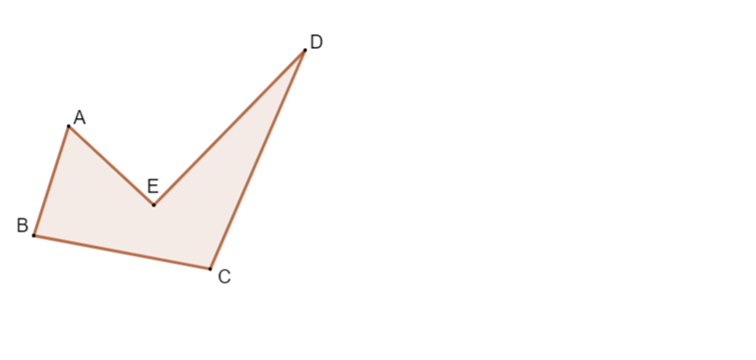
\includegraphics{img/ABCDE.png}
	\end{center}
	\vspace{2cm}
\end{exercise}

\newpage
\begin{exercise}[points=2]
	Trace un triangle $PIE$ si tu sais que $\overline{PI}=5cm$, $\overline{IE}=3cm$ et que la médiane relative à $[PE]$ mesure 4cm.
	\vspace{5cm}
\end{exercise}

\begin{exercise}[points=3]
	Que doit être la valeur de $\bullet$ pour que 358$\bullet$ soit un nombre divisible par 3 et par 4? Laisse tes étapes visibles.
	\vspace{5cm}
\end{exercise}

\end{document}